\chapter{Test 5: Congestion control}
In tasks five and six we study the congestion and its effect on the protocol
performance. In order to provide reliable transport while not contributing to
congestion collapse many protocols provide or use different mechanisms for congestion control and
flow control. In this section we study the effect of heterogeneous bandwidth in
different configurations our protocol implementation supports.

\section{Evaluation scenario}
To evaluate the performance under the assumptions given in this task four clients
were assigned a IP address from loopback address block (127.0.0.0/8). The server
belongs also to this address block. This network setup of ours is given in
figure \ref{fig:task5-setup}.  These additional addresses were created as
alises with command:\\
\\
\texttt{sudo ifconfig lo0 alias 127.0.0.2}
\\

Dummynet was used to create link characteristics between client and server
machines with e.g. following command for each link between client and server
(naturally changing the IP addresses as required): \\ 
\\
\texttt{sudo ipfw add pipe 1 ip from 127.0.0.2 to 127.0.0.10; \\sudo ipfw pipe 1 config bw 500kb }

\begin{figure}
\centering
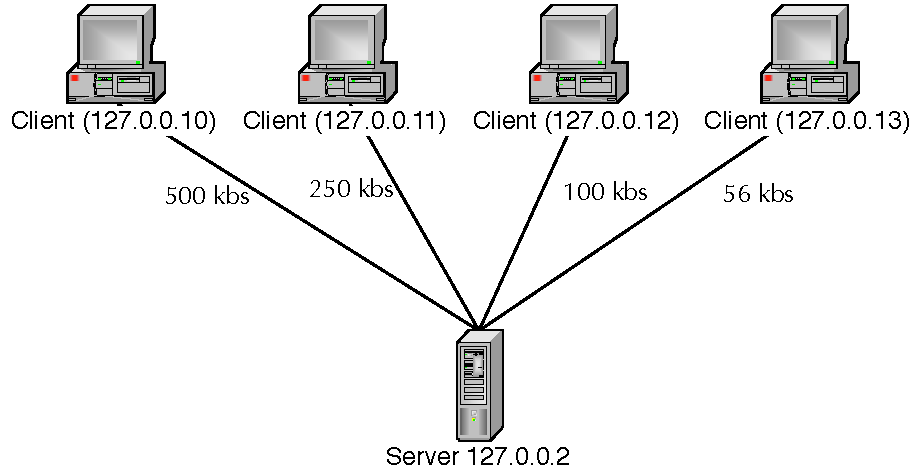
\includegraphics[scale=0.5]{task5-setup.pdf} 
\caption{Number of flows with given flow timeout values}
\label{fig:task5-setup}
\end{figure}

\section{Results}

In table \ref{table:task5-camera-a} the delay statistics and packet loss is
shown for the case where the connections are created without a reliability
guarantees and without any kind of congestion control. 

In table \ref{table:task5-camera-b} the weakly reliable transport is used for
all connections. We see a large increase of packet losses when reliability is
turned on. The reason for this counter intuitive behaviour is most likely due to
camera sensors which have high traffic volumes. In the appendix
\ref{appendix:task5} we see that for low traffic temperature sensors the
weakly reliable transport means less packet losses.

In table \ref{table:task5-camera-c} the results when no reliability guarantees are given but the simple
congestion control mechanism is used.

Finally we show the results when both weakly reliable transport is combined with
simple congestion control in table \ref{table:task5-camera-d}.



In comparison to high traffic volume sensors the results for temperature sensors
are given in appendix.

\begin{table}
\centering
\begin{tabular}{|c|c|c|c|c|c|c|c|c|}
\hline
client & E[D] & max(D) & min(D) & Var(D) & E[s] & max(s) & Var(s) & plr\\
\hline
500kbs & 0.024 & 0.079 & 0 & 0.0001 &  0.067 & 1 & 0.064 & 0\\
\hline
250kbs & 0.047 & 0.100 & 0 & 0.0003 &  0.102 & 1 & 0.093 & 0\\
\hline
100kbs & 0.728 & 1.670 & 0.0199 & 0.186 & 2.203 & 11 & 13.854 & 0.038 \\
\hline
56kbs & 1.935 & 3.950 & 0.0299 & 1.217 & 6.119 & 22 & 48.279 & 0.147 \\
\hline
\end{tabular}
\caption{Task 5: Receive statistics (delay[D], skew[s], packet loss rate [plr]) for camera sensor data (no realibility guarantees, no congestion control)}
\label{table:task5-camera-a}
\end{table}


\begin{table}
\centering
\begin{tabular}{|c|c|c|c|c|c|c|c|c|}
\hline
client & E[D] & max(D) & min(D) & Var(D) & E[s] & max(s) & Var(s) & plr\\
\hline
1 (500kbs) & 0.022 & 0.040 & 0.000 & 0.000 & 0.019 & 1.000 & 0.019 & 0\\
\hline
2 (250kbs) & 0.044 & 0.080 & 0.000 & 0.000 & 0.056 & 1.000 & 0.053 & 0\\
\hline
3 (100kbs) & 0.730 & 2.040 & 0.010 & 0.215 & 3.407 & 34.000 & 41.755 & 0.24\\
\hline
4 (56kbs) & 1.487 & 3.110 & 0.200 & 0.568 & 7.093 & 34.000 & 91.142 & 0.65\\
\hline
\end{tabular}
\caption{Task 5: Receive statistics (delay[D], skew[s], packet loss rate [plr]) for camera sensor data (weakly realible transport, no congestion control)}
\label{table:task5-camera-b}
\end{table}


\begin{table}
\centering
\begin{tabular}{|c|c|c|c|c|c|c|c|c|}
\hline
client & E[D] & max(D) & min(D) & Var(D) & E[s] & max(s) & Var(s) & plr\\
\hline
1 (500kbs) & 0.024 & 0.060 & 0.000 & 0.000 & 0.115 & 1.000 & 0.104 & 0\\
\hline
2 (250kbs) & 0.047 & 0.090 & 0.000 & 0.000 & 0.135 & 1.000 & 0.119 & 0\\
\hline
3 (100kbs) & 0.742 & 1.800 & 0.010 & 0.185 & 2.115 & 12.000 & 12.339 & 0 \\
\hline
4 (56kbs) & 1.972 & 4.090 & 0.020 & 1.085 & 6.231 & 27.000 & 51.985 & 0 \\
\hline
\end{tabular}
\caption{Task 5: Receive statistics (delay[D], skew[s], packet loss rate [plr]) for camera sensor data (no reliability guarantees, skipping messages)}
\label{table:task5-camera-c}
\end{table}


\begin{table}
\centering
\begin{tabular}{|c|c|c|c|c|c|c|c|c|}
\hline
client & E[D] & max(D) & min(D) & Var(D) & E[s] & max(s) & Var(s) & plr\\
\hline
1 (500kbs) & 0.022 & 0.040 & 0.000 & 0.000 & 0.051 & 1.000 & 0.049 & 0\\
\hline
2 (250kbs) & 0.044 & 0.080 & 0.000 & 0.000 & 0.102 & 1.000 & 0.093 & 0\\
\hline
3 (100kbs) & 0.710 & 1.640 & 0.010 & 0.201 & 1.322 & 12.000 & 9.601 & 0.11\\
\hline
4 (56kbs) & 1.356 & 2.760 & 0.020 & 0.718 & 4.000 & 27.000 & 60.690 & 0.59\\
\hline
\end{tabular}
\caption{Task 5: Receive statistics (delay[D], skew[s], packet loss rate [plr]) for camera sensor data (weakly reliable transport, skipping messages)}
\label{table:task5-camera-d}
\end{table}

